% !TeX program = pdflatex
% !TeX encoding = utf8
% !TeX spellcheck = en_GB
% !BIB program = biber

\documentclass[a4paper,parskip=half]{scrartcl}
\usepackage[T1]{fontenc}
\usepackage[utf8]{inputenc}
\usepackage[english]{babel}
\usepackage{amsmath,amssymb,amsfonts}
\usepackage{siunitx}
\usepackage{hyperref}
\usepackage{graphicx}
\usepackage{subfigure}
\usepackage{paralist}

\usepackage{csquotes}
\usepackage[style=authoryear,backend=biber]{biblatex} 
\addbibresource{literature.bib}

\DeclareCiteCommand{\citeyear}
{}
{\bibhyperref{\printfield{year}}}
{\multicitedelim}
{}

\DeclareCiteCommand{\citeyear*}
{}
{\bibhyperref{\printfield{year}\printfield{extrayear}}}
{\multicitedelim}
{}

%opening
\title{Decision Support for Route Planning to Reduce Heat Stress Considering the Time of the Day}
\author{}

\begin{document}

\maketitle

\begin{abstract}
	Heat stress is a serious risk, which affects in particular  groups like elderly or patients with multiple sclerosis or heart disease and is especially pronounced in cities. Developments like the ageing of society, the increasing urbanisation (urban heat island effect) and the climate change are increasing the risk that people are affected by heat stress. One way to reduce those risks is to adapt the everyday behaviour. 
To encourage and support such a change of behaviour, we propose a two step approach. The first step is a route planer for pedestrians that can find a route with minimal heat exposure. The second step is a tool that supports the user to select the point in time with a minimal risk of heat stress, considering e.g. the opening hours of a shop. The route planer is then used to calculate the heat stress and present the optimal route at that point in time.
We evaluate our approach for the city of Karlsruhe. 	
Our results show that the combined approach, as well as only its single steps, can reduce the heat exposure and therefore the heat stress for typical daily tasks.
\end{abstract}

% !TeX encoding = utf8
% !TeX spellcheck = en_GB

\section{Introduction}

Heat is an important factor to human health and comfort. High temperatures cannot only lead to a discomfort, it also has serious negative effects on the health as well as the ability to work. 

In numerous studies an increase in both mortality and
morbidity has been associated with a high ambient temperature \parencite{Basu2009}. The most well-known example in recent history is the 2003 heat wave in Europe. 
Certain groups are especially vulnerable to heat stress such as older people or people with health problems \parencite{Huebler2007}. For patients with multiple sclerosis an increased body temperature can lead to a worsening of their symptoms \parencite{Davis2010}.

Developments like the ageing of society, the increasing urbanisation and the climate change is making the adaptation to heat stress danger more and more important. Due to the tendency that a rising number of people is moving into the cities, the urban heat island effect (UHI) is gaining more importance in the future. The UHI effect states that an urban area is significantly warmer than surrounding rural areas \parencite{Prashad2014}. 

Individuals can reduce their heat stress by adapting their everyday behaviour. In a city, most typical activities are in walking distance. These can range from going to a grocery store to the visit of a doctor. While these activities cannot be omitted, it is possible to use different routes or change the time when they are conducted. In doing so, one can easily reduce the heat stress without negative impact on the quality of life. 

In this paper we use this reasoning into a two-step approach to help individuals reduce their heat stress. We apply a routing algorithm to compute the optimal path in regard to the heat stress. This algorithm is then used to determine the optimal point in time to conduct typical everyday activities. 
  
\subsection{Related Work} 

\subsubsection{Heat Stress}
The impact of heat on the human body has long been a subject of study. Thermal comfort plays a key role, which describes climatic conditions consider comfortable. 

\textcite{Staiger1997} state that only a complete heat budget model of the human body is sufficient to make any reliable statements regarding the influence of heat on the body. Some well-known indices that consider a complete human heat budget model are for instance:
\begin{inparaenum}[(1)]
  \item \citeauthor{Steadman1979}'s heat index (\citeauthor{Steadman1979} \citeyear*{Steadman1979}, \citeyear*{Steadman1979a}),
  \item the predicted mean vote (PMV) \parencite{Fanger1973},
  \item the perceived temperature \parencite{Staiger1997,Jendritzky2000},
  \item and the universal thermal climate Index UTCI \parencite{Jendritzky2010}.
\end{inparaenum}

For all these indices the following meteorological parameters are important:
\begin{inparaenum}[(1)]
\item air temperature,
\item water vapour pressure,
\item wind velocity 
\item and mean radiant temperature \parencite{Jendritzky2010}.
\end{inparaenum}

Based on the availability of data, in this paper we will use \citeauthor{Steadman1979}'s heat index \parencite{Steadman1979} and, as a simple comparison measure, the air temperature.

\subsubsection{Health Optimal Pedestrian Routing}
Several research projects have considered environmental factors for pedestrian routing in the past, with the goal to find routes which are healthier. For instance, \textcite{Sharker2012} are proposing a method to find a health optimal route, considering several environmental factors like complexity of the walking trail and weather. A method to find a route with a minimal pollution exposure has been proposed by \textcite{Hasenfratz2015}.

The NaviComf framework for pedestrian routing proposed by \textcite{Dang2013} improves the comfort considering environmental factors varying over time. Their  framework uses a multi-factor cost model for the evaluation of the route and enables a consideration of heterogeneous environmental information from multi-modal sensors. To find an optimal route \textcite{Dang2013} are proposing three different algorithms, a bounded depth-first search algorithm, an adjustable dynamic planning algorithm and a heuristic particle planning algorithm. As a sample application, the authors implemented a routing application for thermal comfort navigation. The meteorological data used for this sample application have been collected using a network of 40 micro-climate sensor nodes which detected air temperature and relative humidity. 

In contrast to the existing work, we contribute an approach which does not rely on extensive sensor networks. We achieve this by combining remote sensing data with fixed weather stations and the use of a static routing algorithm.
% !TeX encoding = utf8
% !TeX spellcheck = en_GB

\section{Minimize Heat Exposure}

We are presenting a two-step approach to supported people to reduce their heat stress in their everyday life. First we are presenting an approach to find a route for pedestrian with a minimal heat exposure. On this basis, we show an approach to find a point in time with a minimal heat exposure, for instance to go shopping in a supermarket.

\subsection{Finding a Route with Minimal Heat Exposure}

\subsubsection{Modelling as a Time-Dependent Routing Problem}

Finding a route with minimal heat exposure can be modelled as time-dependent routing problem, where the edge weighting function is not static and instead may vary over time. Subsequently, many speed up techniques developed for static routing problems like bi-directional search cannot simply be applied \parencite{Delling2009}. 

Below, we are representing the road network as undirected graph $G=(V,E,w_d,w_h)$, where $V$ is the set of vertices or nodes (e.g. junctions) and $E\subseteq V\times V$ is the set of edges (e.g. road segments) each connecting a pair of nodes. Furthermore $w_d: E \to \mathbb{R}_{\geq 0}$ and $w_h: E \times T \to \mathbb{R}_{\geq 0}$ are to edge weighting function, at which:
\begin{itemize}
	\item $w_d(e)$ is the length of the edge $e$, and
	\item $w_h(e, t)$ is the heat exposure of edge $e$ at time $t$.
\end{itemize}   
Hereafter, a path $p$ from node $v_0$ to node $v_k$ starting a time $t_0$ is denoted as sequence of edge-time pairs $((e_{v_0v_1},t_0),(e_{v_1v_2},t_1),\dots, (e_{v_{k-1}v_k},t_{k-1}))$, where $t_i$ is the time at which node $v_i$ is leaved. The weight of an edge is fixed at the time the traversing of the edge is started \parencite[the so-called frozen link model,][]{Orda1990}. The time $t_i$ can be computed as follows: $t_i := t_{i-1} + t_{walk}(e_{v_{i-1},v_i})$ where $t_{walk}(e_{v_{i-1},v_i})$ is the time needed by a pedestrian to traverse the edge $e_{v_{i-1},v_i}$. The starting time $t_0$ is ether given or set to~$0$. 

To compute the weight of a path $w_h(p)$ the following formula can be applied:
	\begin{equation}\label{eq:path-weight}
		w_h(p) := \sum_{(e,t) \in p} w_h(e, t).
	\end{equation}
Those means we are looking for the path $p^*$ from a node $v$ to a node $u$ that has the minimal weight of all possible path from $v$ to $u$. Below, we are using $w_h(p, t)$ to denote the weight of the path $p$ starting at time $t$. 

The time-dependent routing problem is $\mathcal{NP}$-hard, if it is not allowed to wait on a node and the FIFO (first in, first out) property is not fulfilled \parencite{Orda1990}. A weighting function $w$ fulfils the FIFO property if the numerator (change of the edge weight) decreases not faster than the denominator (change in actual time) increases \parencite{Kaufman1993}. 

Usually, we cannot assume that $w_h$ fulfils the FIFO property, because the function most of the time depends on the air temperature and the air temperature can decrease more than actual time increases. Since, most people are not willing to wait at a node as well, finding a route with a minimal heat exposure is $\mathcal{NP}$-hard. Therefore, 
hereafter the edge weighting is frozen at the starting time $t_0$ so that we have static route planning problem and classic algorithms like  \citeauthor{Dijkstra1959}'s algorithm \parencite{Dijkstra1959} can be applied. 



\subsubsection{The Edge Weighting Function \label{sec:edge-weighting}}

\begin{figure}
	\centering
	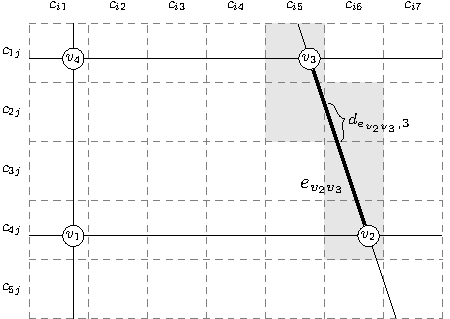
\includegraphics{figures/raster-edge-mapping-standalone}
	\caption[Example for the raster to edge mapping]{An 
		example for the raster to edge mapping.}
	\label{fig:raster-edge-mapping}
\end{figure}

To find a route with a minimal heat exposure it is key to define the edge weighting function in an appropriated way. At this, it is not sufficient to only take the actual thermal comfort in to account, we also must consider the time a person is exposed to heat. Below, we assume that the time of exposure is proportional to the length of the edge $w_d$ \parencite[following][]{Hasenfratz2015}. Based on this assumption we are defining the edge weighting function $w_h$ as follows: 
\begin{equation}\label{eq:edge-weight}
w_h(e, t) := \sum_{c \in Intersec(e)} d_c \cdot h_c(t).
\end{equation}
Here, the thermal comfort values (like air temperature or heat index) are represented as time-dependent raster $H(t) = \left(h_{ij}(t)\right)$, where $h_{ij}(t)$ denotes the thermal comfort value in raster cell $c_{ij}$ at time $t \in T$. In the formula above, $Intersec(e)$ is the set of raster cells intersected by the edge $e$ and $d_c$ the length of the intersection of $e$ with raster cell $c$.  That is, to obtain the edge weight, the value of each intersected raster cell is weighted with the length of the intersection and then accumulated, as shown in figure~\ref{fig:raster-edge-mapping}.

Using the actual thermal comfort measures -- air temperature and heat index -- we get the following edge weighting functions:
\begin{align}
	\label{eq:edge-weight-temperature}
	w_{T_a}(e,t)& = \sum_{c \in Intersec(e)} d_c \cdot T_a(t, c),
\end{align}
for the air temperature and respectively:
\begin{align}
	\label{eq:edge-weight-heatindex}
	w_{HI}(e,t)& = \sum_{c \in Intersec(e)} d_c \cdot T_{HI}\left(T_a(t, c), RH(t)\right)
\end{align}
for the heat index. Here, $T_a(t,c)$ is the air temperature in raster cell $c$ at time $t \in T$, $RH(t)$ is the relative humidity at time $t$ and $T_{HI}$ is Steadman's heat index. How we obtained those values is described below in section \ref{sec:data-sets}.

 \subsection{Finding the Optimal Time \label{sec:find-optimal-time}}
 
 Apart from selecting a route with minimal heat exposure the risk of heat stress in the everyday life (e.g. go shopping in a supermarket) can massively be reduced by selecting the appropriate time for this action. That's because usually, the heat exposure is highest at middays and significant lower in the morning or evening.
 
 To give recommendations for a time with minimal heat exposure, we are use a three step procedure: 
 
 \begin{enumerate}
 	\item \label{itm:nearby-search} Perform a nearby search originating from a given starting point $s$  (e.g. address or GPS coordinates) to find all locations $L$ that fulfils a certain search criteria (e.g. is supermarket or pharmacy)  within a specified radius $r$ (e.g. \SI{500}{\meter}).
 	
 	\item \label{itm:optimal-time} For each location $\ell \in L$ found in step \ref{itm:nearby-search}, determine the point in time $t^*$ with the lowest heat exposure. 
 	
 	\item \label{itm:ranking} Create a ranking of the locations in $L$ based on the minimum heat exposure found in step \ref{itm:optimal-time}, so that the location with the lowest heat exposure has rank 1.
 \end{enumerate} 

The steps \ref{itm:nearby-search} and \ref{itm:ranking} are not very complicated, so we are focusing on step \ref{itm:optimal-time}. 

\subsubsection{Modelling as a Optimization Problem} 

If we are search for the optimal time for a location $\ell \in L$ we should consider certain constrains like the opening hours $[t_{open}(\ell),t_{close}(\ell)]$ of $\ell$. As the objective function to minimize we are using the heat exposure of the optimal path between the starting point $s$ and a location $\ell$ as proposed above. Those, finding the time with the minimal heat exposure means to minimize the following objective function $h(\ell, t)$:
	\begin{equation}\label{eq:objective-funtion}
		h(\ell, t) = w_h(p^*, t) = \min_{p\in P_{s\ell}} w_h(p, t) = \min_{p\in P_{s\ell}} \sum_{(e, t') \in p} w_h(e, t'),
	\end{equation}
where $P_{s\ell}$ is the set of all possible paths from $s$ to $\ell$,  $w_h(p, t)$ is the accumulated edge weight of all edges in $p$ at starting time $t$ and $w_h$ is the edge weighting function from equation \eqref{eq:edge-weight}. 

Using the objective function defined in equation \eqref{eq:objective-funtion}, we can formulate the problem to find a time with minimal heat exposure as a optimization problem with constrains:
\begin{subequations}
	\label{eq:optimal-time}
	\begin{alignat}{2}
	&\min_{t \in T} h(\ell, t) && \label{eq:optimal-time:of} \\
	%& \text{s.t.} &  t_{open}(\ell)  \leq t &\leq t_{close}(\ell) \label{eq:optimal-time:oh} \\
	&\text{s.t.} & t & \geq t_{open}(\ell)-t_{walk}(\ell, t) \label{eq:optimal-time:twm}\\
	&	& t & \leq   t_{close}(\ell)-(t_{walk}(\ell, t)+t_{buff}(\ell))	\label{eq:optimal-time:twe}\\
	&	&  t & \geq t_{earliest} \label{eq:optimal-time:te} \\
	&	&  t & \leq t_{latest} \label{eq:optimal-time:tl} \\
	&  & t  & \geq t_{now} \label{eq:optimal-time:tn} 
	\end{alignat}
\end{subequations}

Note, that the location $\ell$ is fixed, the selection of the location with lowest heat exposure is performed later in step \ref{itm:ranking}. The constrains \eqref{eq:optimal-time:twm} and \eqref{eq:optimal-time:twe} are  basically ensuring that the location is arrived within the opening hours. We must ensure that the shop can be reached before it closes, therefore we have to consider the time needed to walk to the location $\ell$ ($t_{walk}(\ell)$) as well as the time needed to perform e.g. the purchase ($t_{buff}(\ell)$). On the other hand, it can make sense to start early in the morning  arrive the location $\ell$ just in time when its opening, so we are subtracting the walking time from the opening time. The constrains \eqref{eq:optimal-time:te} and \eqref{eq:optimal-time:tl} are an earliest respectively latest time desired by the user and can be omitted. Finally, the last constrain  \eqref{eq:optimal-time:tn}  guarantees, that the optimal time is in the future. Another thing to notice is, that the walking time $t_{walk}(\ell, t)$ depends on the starting time $t$, because conditional on the time a different (properly longer) optimal route can be selected.

 \subsubsection{Optimization \label{sec:optimization}}
 
 To find the optimal time, we need a optimization method without derivatives, because the objective function $h(\ell, t)$ is not necessarily derivable. One such method is Brent's method \parencite{Brent2002}, a procedure for the approximation of local optima within an interval $[x_1, x_2]$.
 
 In order to apply Brent's method, we have to transform the constrains \eqref{eq:optimal-time:twm} -- \eqref{eq:optimal-time:tn} to a lower and upper limit of an interval.  The constrains \eqref{eq:optimal-time:twm}, \eqref{eq:optimal-time:te} and \eqref{eq:optimal-time:tn} can  be easily converted to a lower limit, as follows: 
  	\begin{equation}\label{eq:lower-limit}
  		t_{lower}(\ell, t) = \max\left\lbrace  t_{open}(\ell)-t_{walk}(\ell, t), t_{now}, t_{earliest} \right\rbrace.
  	\end{equation}
  Alike, we can transform the constrains \eqref{eq:optimal-time:twe} and \eqref{eq:optimal-time:tl} to an upper limit:
  	\begin{equation}\label{eq:upper-limit}
  		t_{upper}(\ell, t) = \min\left\lbrace  t_{close}(\ell)- (t_{walk}(\ell, t) + t_{buff}(\ell)), t_{latest} \right\rbrace.
  	\end{equation}
 It's simple to recognize, that the interval $[t_{lower}(\ell, t), t_{upper}(\ell, t)]$ preserves the constrains from the optimization problem defined above in equation \eqref{eq:optimal-time}.  
 
 However, Brent's method can still not be applied, since -- as outlined above in section \ref{sec:optimization} -- the lower and upper limit of the interval is depending on the starting time $t$ and therefore, not static as required for Brent's method. As solution to avoid this problem we are proposing the introduction of a penalty term:
 \begin{equation}
 \label{eq:optimal-time-penality}
 h'(t,\ell) = \begin{cases}
 h(t,\ell) & \text{if }t_{open}(\ell)-t_{walk}(\ell,t) \leq t \leq  t_{close}(\ell)-(t_{walk}(\ell,t)+t_{buff}(\ell)),\\
 h(t,\ell)  + c & \text{otherwise,}
 \end{cases}
 \end{equation}
 where $c$ is a large constant such that $h(t,\ell) + c$ is never selected as optimal solution, if the constrains are violated. Now, we can use the walking time $t_{walk}^{shortest}(\ell)$  for the shortest route for the lower and upper limit. Finally, we can formulate the optimization problem for Brent's method as follows:
 \begin{subequations}
 	\label{eq:brent-optimization-problem}
 	\begin{alignat}{2}
 	&\min_{t \in T} h'\ell, t) && \\
 	&\text{s.t.} & t & \geq \max\left\lbrace  t_{open}(\ell)-t_{walk}^{shortest}(\ell), t_{now}, t_{earliest} \right\rbrace \\
 	& & t &\leq \min\left\lbrace  t_{close}(\ell)- \left(t_{walk}^{shortest}(\ell) + t_{buff}(\ell)\right), t_{latest} \right\rbrace.
 	\end{alignat}
 \end{subequations}
Now we can use Brent's method to find for each location $\ell$ the optimal time $t^*$. To avoid, that the Brent optimizer is trapped in a local optimum, its executed several times with different random start points.

% !TeX encoding = utf8
% !TeX spellcheck = en_GB

\section{Evaluation}

\subsection{Data}
\label{sec:data-sets}
As map data, we use the OpenStreetMap (OSM) project \parencite{OSMF2016}. 
For temperature data we use the hourly air temperature and relative humidity values are originating from the weather station of the German Weather Service (Deutscher Wetterdienste, DWD) in Rheinstetten near Karlsruhe \parencite{DWD2016}. For a finer spatial resolution we use remote sensing data of a thermal scanner flight provided by the Nachbarschaftsverband Karlsruhe (NVK). The data set consists of two scans, recorded in the morning and in the evening of the 26 September 2008. The data are covering an area of  $\SI{25 805}{\meter} \times \SI{39 555}{\meter}$ (EW NS) and have a resolution of $5\,161 \times 7\,911$  pixels. The measured surface temperature is in the range of \SIrange{-1.7}{18.3}{\celsius} (morning and evening). The average surface temperature of the cropped data sets has been \SI{4.18}{\celsius} (morning) respectively \SI{11.24}{\celsius} evening.  


\subsection{Data Preparation}
First, the OSM data set is cropped to the evaluated area. Afterwards, all ways tagged with \verb|highway|, \verb|railway=platform| or \verb|public_transport=platform| are extracted to obtain the road network.

To compute the edge weights as described above in section \ref{sec:edge-weighting} we need to make some assumptions. That's because the weather data that we use lack either an appropriate spatial resolution or the required temporal resolution. We assume that the actual spatial variation of the temperature conforms with the spatial variation of the thermal scans (deviation from the mean value). For the relative humidity, we assume a constant value over the study area. For the temporal variation, we assume that the temporal variation in the examined area corresponds to the temporal variation measure at the weather station. We apply the morning scan to timestamps between  00:00 and 11:59 and the evening scan between 12:00 and 23:59.

We compute the air temperature at time $t\in T$ for the raster cell $c_{ij}$ as follows:
\begin{equation}
\label{eq:derived-temperature}
T_a(t, c_{ij}) = \begin{cases}
T_{a}^{station}(t) + \delta_{ij}^{morning} & \text{if $0 \leq t < 12$,}\\
T_{a}^{station}(t) + \delta_{ij}^{evening} & \text{if $12 \leq t < 24$,}
\end{cases}
\end{equation}
where $T_{a}^{station}(t)$ is the air temperature measured at the weather station at time $t$ and $\delta^{morning}_{ij}$ respectively  $\delta^{evening}_{ij}$ is the deviation of the raster cell $c_{ij}$ from the mean of all raster cells from the morning respectively evening scan.

We compute an approximation of Steadman's heat index with \textcite[77]{Stull2011}. Since the heat index is only defined for an air temperature between \SI{20}{\celsius} and \SI{50}{\celsius} we use the air temperature as a fall-back value. If the air temperature drops in a raster cell below a comfort threshold $T_a^{comfort}$ or $T_{HI}^{comfort}$, then that comfort value will be used, because temperature below this threshold are not considered harmful. 

For the implementation of the routing we used the GraphHopper framework for Java \parencite{GraphHopper2016}.


To find an optimal point in time we used the procedure described in section \ref{sec:find-optimal-time}.  

For the nearby search, we  use a list of selected OSM tags like \verb|shop=supermarket| or \verb|amenity=pharmacy| as a search criteria. We also only consider locations which have opening hours specified (via the \verb|opening_hours| tag). Additionally, only locations which are in a defined radius around the starting point are considered, at this we use the direct distance (“as the crow flies”). To reduce the computation effort a maximum number of results $k$ can be specified.

As optimization algorithm, we use the implementation of Brent's method in the Apache Commons Mathematics Library \parencite{ASF2016} with 10 random start points to reduce the risk that only a local optimum is found.

\subsection{Results}

\subsubsection{Routing}

\begin{table}
	\centering
	\begin{tabular}{lp{9.25cm}lcc}
		\toprule
		& & temperature & heat index \\
		\midrule
		\multicolumn{4}{l}{Reduction of heat exposure (\% of cases) }   \\
		& overall  & \SI{79.70}{\percent} & \SI{80.53}{\percent}  \\
		& more then \SI{5}{\percent} & \SI{42.72}{\percent} & \SI{45.11}{\percent} \\
		& more then \SI{10}{\percent} & \SI{13.81}{\percent} & \SI{16.07}{\percent} \\
		\multicolumn{4}{l}{Reduction of heat exposure}  \\
		& average  & \SI{4.63}{\percent} & \SI{4.69}{\percent}  \\
		& maximum  & \SI{25.97}{\percent} & \SI{26.17 }{\percent}  \\
		\multicolumn{4}{l}{Increase of distance}  \\
		& average & \SI{5.59}{\percent} & \SI{5.76}{\percent}  \\
		\multicolumn{4}{l}{Reduction of relative heat exposure ($w_h / w_d$)}  \\
		& average  & \SI{2.12}{\celsius} & \SI{2.32}{\celsius}  \\
		\bottomrule
	\end{tabular}
	\caption{Overview of the routing results. The values are relative to the shortest route. \label{tab:results-routing}}
\end{table}

\afterpage{
\begin{figure}
	\centering
	\subfigure[map]{
		\label{fig:route-example:map}
		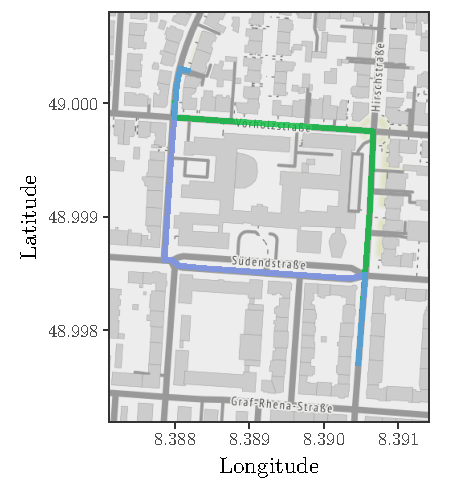
\includegraphics[scale=0.7]{figures/route_example_map}
	}    
	\subfigure[thermal scan (evening)]{
		\label{fig:route-example:raster}
		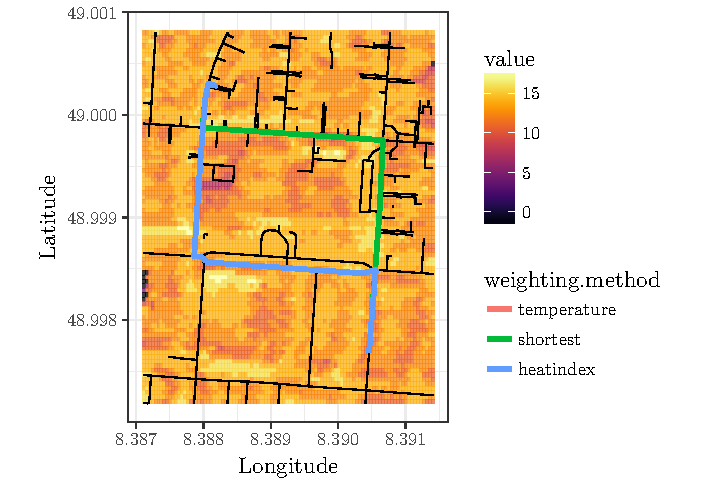
\includegraphics[scale=0.7]{figures/route_example_raster}
	}     
	\caption{Routing example: both the \emph{temperature} and the \emph{heatindex} weighting found the same route. (Map tiles by \textcite{Stamen2017}, under CC BY 3.0\protect\footnotemark{}. Map data by \textcite{OSMF2016}, under ODbL\protect\footnotemark{})}
	\label{fig:route-example}
\end{figure}
\addtocounter{footnote}{-1}
\footnotetext{\url{http://creativecommons.org/licenses/by/3.0}}
\stepcounter{footnote}
\footnotetext{\url{http://www.openstreetmap.org/copyright}}
}

To evaluate the routing, we select 1000 random pairs of start and destinations points form the examined  area and 10 random dates from the period of 1 June to 31 August 2015. For each of the start destination pairs and each date we  perform the evaluation at 7:00, 11:00, 15:00, 19:00 and 23:00, so overall we had $50\,000$ samples. As benchmark we computed for each sample the shortest path. 


An overview of our results is given in table \ref{tab:results-routing}. In many cases the heat exposure could be reduced. On average the heat exposure has been decreased by \SI{\sim 4.7}{\percent} while in the same time the distance was increased by at most \SI{5.76}{\percent} on average. In some cases, the heat exposure can be reduced by up to \SI{25}{\percent}. The weighted average of the thermal comfort measure can be reduced by \SI{\sim 2}{\celsius} on average. There are only slight differences between the air temperature and the heat index as measure for thermal comfort. 

In the example given in figure \ref{fig:route-example} the heat exposure could be reduced by \SI{17.64}{\percent} (\emph{temperature}) and \SI{18.76}{\percent} (\emph{heatindex}), while at the same time the distance only increased by  \SI{0.53}{\percent}.

\subsubsection{Optimal Time}

\begin{table}
	\centering
	\begin{tabular}{lp{9.25cm}lcc}
		\toprule
		& & temperature & heat index \\
		\midrule
		\multicolumn{4}{l}{Reduction of heat exposure}   \\
		& \% of cases  & \SI{68.43}{\percent} & \SI{71.08}{\percent}  \\
		\multicolumn{4}{l}{Reduction of heat exposure}  \\
		& average  & \SI{8.09}{\percent} & \SI{7.73}{\percent}  \\
		& maximum  & \SI{62.29}{\percent} & \SI{62.88}{\percent}  \\
		\multicolumn{4}{l}{Increase of distance}  \\
		& average  & \SI{4.60}{\percent}  & \SI{4.72}{\percent}  \\
		\bottomrule
	\end{tabular}
	\caption{Overview of the results of the combined approach each compared with the reference solution.  \label{tab:results-optimal-time}}
\end{table}

\begin{figure}
	\centering
	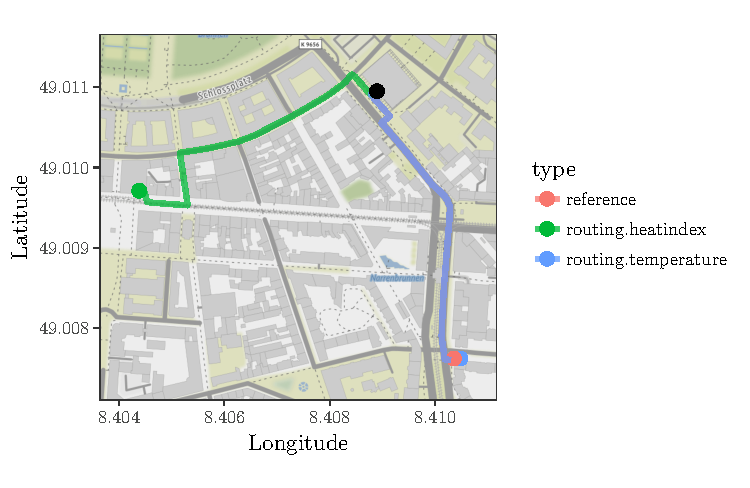
\includegraphics[scale=1]{figures/optimaltime_route_example}
	\caption{Example for nearby search: In the graphic the starting point (black dot) as well as the locations ranked first by the respective method. (Map tiles by \textcite{Stamen2017}, under CC BY 3.0. Map data by \textcite{OSMF2016}, under ODbL)}
	\label{fig:optimaltime-route-example}
\end{figure}

For the evaluation of optimal time finding procedure we selected 750 random start points. One of the following four search criteria has been assigned to each of the start points at random: supermarket, bakery, chemist or pharmacy. For each of the start points a random start time $t_{now}$ has been selected from the period of 8:00 to 20:00. The radius has been set to \SI{1000}{\meter} for all start points and the maximum number of results has been set to 5. Additionally, for all start points a time buffer $t_{buff}$ of 15 minutes has been assumed. 

As a reference solution, we use the closest location found during the nearby search, compute the shortest path from the starting point to this location and evaluated the heat exposure at time $t_{now}$. 

The results for the combined approach are given in table \ref{tab:results-optimal-time}. Here the average reduction compared to the routing approach is significantly higher. This is expected as the heat exposure can vary strongly with the time of the day. 

In the example given in figure \ref{fig:optimaltime-route-example} the \emph{temperature} weighting selected the same pharmacy and optimal point in time (9:27) as the reference solution. Contrary the \emph{heatindex} weighting selected a different pharmacy which is \SI{476.6}{\meter} instead of  \SI{434.5}{\meter} away from the start. Additional the method found a different optimal time (19:39) and those the heat exposure could be reduced by \SI{18.49}{\percent}.  
 

% !TeX encoding = utf8
% !TeX spellcheck = en_GB

\section{Conclusion}

In this work, we proposed a two-step approach to reduce the heat stress for individuals. We achieved this goal by creating a decision support system that computes heat-optimal paths to locations as well the optimal points in time to do so. We evaluated this on typical every-day activities such as grocery shopping. 
We showed that our approach reduces the heat stress in a vast majority of the cases. On average the heat stress can be reduced by \SI{\sim 4.7}{\percent} while the trade off in additional distance is also quite low. This is never more than \SI{5.76}{\percent} on average. We achieved these results, contrary to the existing work, for relatively small distances which average over \SI{\sim  2}{\kilo\meter}.
The impact of these results are simple, but significant. One can easily compute our approach and decide for themselves the trade-off between additional distance and the heat stress reduction.
Thanks to the very small assumptions on the data set, one can apply the approach quite easily to other cities. 
But these assumptions are also the main restriction of this work. Given the rise of smart cities and (hopefully) more available data sources, one could improve the approach with more fine-detailed data. Even more interesting would be the inclusion of intra urban temperature forecasts. By incorporating exact forecasts of future values along possible pathways, the optimal point in time as well as the reduction of the heat stress could be improved. Additionally, the inclusion of more complex heat indices could increase the validity for any potential user. 
Finally, the computation of an overall route which covers a multitude of potential points of interests would be an interesting extension. This could be used for tourists or even worker scheduling. Here not only the time and the route with minimal heat exposure should be considered but also, the ordering of the locations.  
%% !TeX encoding = utf8
% !TeX spellcheck = en_GB

\section{Story}
\begin{itemize}
	\item Motivation
	\begin{itemize}
		\item heat is critical for humans
		\item particular problems for risk groups (illness, old, etc)
		\item walking to areas often done action in particular to typical locations (shopping, health care, etc)
		\item those actions have to be done   
	\end{itemize}
	\item Problem definition
	\begin{itemize}
		\item how to minimize the impact of heat stress on walking paths?
		\item subdivided into:
		\begin{itemize}
			\item for a given route?
			\item When and how to walk typical routes, e.g. pharmacy, doctor
		\end{itemize} 
	\end{itemize}
	\item method:
	\begin{itemize}
		\item Goal of this paper: We want to provide a routing method to minimize the heat stress of typical walking actions
		\item We do so by providing a value function for heat stress which can be used in route planning
	\end{itemize}
	\item Evaluation:
	\begin{itemize}
		\item Our data set
		\item Evaluation 1 on routes given date in time.  (pure routing approach) and its metrics
		\item Evaluation 2: producing queries for typical walking tasks (our selection) and their evaluation
		\item implementation as a demonstrator is produced and available at $homepage$
	\end{itemize}
	\item Conclusion and contribution
\end{itemize}


 


\printbibliography

\end{document}
